\documentclass[final]{beamer}

\usepackage[scale=1.24]{beamerposter} % Use the beamerposter package for laying out the poster

\usepackage{siunitx}

\usetheme{confposter} % Use the confposter theme supplied with this template

\setbeamercolor{block title}{fg=nblue,bg=white} % Colors of the block titles
\setbeamercolor{block body}{fg=black,bg=white} % Colors of the body of blocks
\setbeamercolor{block alerted title}{fg=white,bg=dblue!70} % Colors of the highlighted block titles
\setbeamercolor{block alerted body}{fg=black,bg=dblue!10} % Colors of the body of highlighted blocks
% Many more colors are available for use in beamerthemeconfposter.sty

\usepackage[skins]{tcolorbox}
% a "sub-block" (plain block-within-block (second-level header))
\newenvironment{subblock}[1]{
  \setbeamertemplate{block begin}
  {
    \setbeamercolor{block title}{fg=nblue!90} % @TODO defer to beamercolortheme
    \par\vskip\medskipamount
    \begin{beamercolorbox}[colsep*=0ex,dp={2ex}]{block title}
      \vskip-0.5cm
      \begin{tikzpicture}[every node/.style={inner sep=0}]
        \node (titlenode) at (0.1cm, 0) {\usebeamerfont{block title}\normalsize\insertblocktitle};
        \tcbsetmacrotowidthofnode{\titlewidth}{titlenode}
        \tcbsetmacrotoheightofnode{\titleheight}{titlenode}
        \shade [inner color=nblue!16!black!24,outer color=white]
        (-\titlewidth/2,-\titleheight/2) rectangle ++({1.1*\titlewidth+0.1cm},-0.2cm);
      \end{tikzpicture}
    \end{beamercolorbox}
    {\parskip0pt\par}
    \ifbeamercolorempty[bg]{block title}
    {}
    {\ifbeamercolorempty[bg]{block body}{}{\nointerlineskip\vskip-0.5pt}}
    \usebeamerfont{block body}
    \vskip-0.5cm
    \begin{beamercolorbox}[colsep*=0ex,vmode]{block body}
      \justifying
    }
    \setbeamertemplate{block end}
    {
    \end{beamercolorbox}
    \vskip\smallskipamount
  }
  \begin{block}{{\normalsize #1}}
  }{\end{block}}

\newlength{\sepwid}
\newlength{\colonewid}
\newlength{\coltwowid}
\newlength{\colthreewid}
\setlength{\paperwidth}{48in} % A0 width: 46.8in
\setlength{\paperheight}{36in} % A0 height: 33.1in
\setlength{\sepwid}{0.024\paperwidth} % Separation width (white space) between columns
\setlength{\colonewid}{0.29\paperwidth} % Width of column one
\setlength{\coltwowid}{0.324\paperwidth} % Width of column two
\setlength{\colthreewid}{0.29\paperwidth} % Width of one column
\setlength{\topmargin}{-0.5in} % Reduce the top margin size
% -----------------------------------------------------------

\usepackage{graphicx}  % Required for including images
\usepackage{booktabs} % Top and bottom rules for tables
\usepackage{tikz}
\usetikzlibrary{
  arrows,
  calc,
  decorations.pathmorphing,
  decorations.pathreplacing,
  decorations.markings,
  fadings,
  positioning,
  shapes,
  arrows.meta
}
\usepgfmodule{oo}

\pgfdeclareradialshading{glow2}{\pgfpoint{0cm}{0cm}}{
  color(0mm)=(white);
  color(2mm)=(white);
  color(8mm)=(black);
  color(10mm)=(black)
}
\pgfdeclareradialshading{glow}{\pgfpoint{0cm}{0cm}}{
  color(0mm)=(white);
  color(5mm)=(white);
  color(9mm)=(black);
  color(10mm)=(black)
}

\begin{tikzfadingfrompicture}[name=glow fading]
  \shade [shading=glow] (0,0) circle (1);
\end{tikzfadingfrompicture}

\begin{tikzfadingfrompicture}[name=glow2 fading]
  \shade [shading=glow2] (0,0) circle (1);
\end{tikzfadingfrompicture}

\definecolor{atomorange}{rgb}{1.0,0.483,0.0}
\definecolor{pyplotc0}{rgb}{0.122,0.467,0.706}
\definecolor{pyplotc1}{rgb}{1.000,0.498,0.055}
\definecolor{pyplotc2}{rgb}{0.173,0.627,0.173}
\definecolor{pyplotc3}{rgb}{0.839,0.153,0.157}
\definecolor{pyplotc4}{rgb}{0.580,0.404,0.741}
\definecolor{pyplotc5}{rgb}{0.549,0.337,0.294}
\definecolor{pyplotc6}{rgb}{0.890,0.467,0.761}
\definecolor{pyplotc7}{rgb}{0.498,0.498,0.498}
\definecolor{pyplotc8}{rgb}{0.737,0.741,0.133}
\definecolor{pyplotc9}{rgb}{0.090,0.745,0.812}

\pgfdeclarelayer{tweezer}
\pgfsetlayers{tweezer,main}
\pgfooclass{tweezer}{
  \method tweezer() {
  }
  \method drawAtom(#1,#2,#3,#4) {
    \fill [#4,path fading=glow2 fading] (#1,#2) circle (#3);
  }
  \method drawDownAtom(#1,#2,#3) {
    \pgfoothis.drawAtom(#1,#2,#3,pyplotc0);
  }
  \method drawUpAtom(#1,#2,#3) {
    \pgfoothis.drawAtom(#1,#2,#3,pyplotc1);
  }
}
\pgfoonew \mytweezer=new tweezer()



% --------------------------------------------------------------------------------
%	TITLE SECTION
% --------------------------------------------------------------------------------

\def\realtitle{Mid-circuit measurement on $^{171}$Yb$^+$ using the \textit{omg} architecture}

\title{%
  \texorpdfstring{%
    \makebox[\linewidth]{%
      \makebox[0pt][l]{%
        \raisebox{\dimexpr-\height+0.5\baselineskip}[0pt][0pt]
        {
          \begin{tikzpicture}
            \node at (0, 0) {
\includegraphics[width=15cm]{imgs/logos/Duke}};

            \node at (11.5, 0) {
\includegraphics[width=4cm]{imgs/logos/ARL}};
          \end{tikzpicture}
        }% Left logo
      }\hfill
      \makebox[0pt]{\textcolor{dblue}{\realtitle}}%
      \hfill\makebox[0pt][r]{%
        \raisebox{\dimexpr-\height+0.5\baselineskip}[0pt][0pt]
        {
          \begin{tikzpicture}
            \node at (0, 0) {
\includegraphics[width=6.5cm]{imgs/logos/NIST}};
            \node at (7.5, 0) {
\includegraphics[width=6.5cm]{imgs/logos/Sandia}};
            \node at (2.25, -5) {
\includegraphics[width=8cm]{imgs/logos/ColdQuanta2}};
          \end{tikzpicture}
        }% Right logo
      }%
    }%
  }
  {\realtitle}} % Poster title

\author{Yichao Yu\inst{1}, Keqin Yan\inst{1}, Debopriyo Biswas\inst{1},
  Vivian Zhang\inst{1}, Bahaa Harraz\inst{1},\\
  Marko Cetina\inst{1}, Crystal Noel\inst{1}, Alexander Kozhanov\inst{1},
  Christopher R Monroe\inst{1}}
\institute{\inst{1} Duke Quantum Center, Duke University}

\ifpdf
  % Ensure reproducible output
  \pdfinfoomitdate=1
  \pdfsuppressptexinfo=-1
  \pdftrailerid{}
  \hypersetup{
    pdfcreator={},
    pdfproducer={}
  }
\fi

\begin{document}

\addtobeamertemplate{block end}{}{\vspace*{2ex}} % White space under blocks
\addtobeamertemplate{block alerted end}{}{\vspace*{2ex}} % White space under highlighted (alert) blocks

\setlength{\belowcaptionskip}{2ex} % White space under figures
\setlength\belowdisplayshortskip{2ex} % White space under equations

\definecolor{trapyellow}{HTML}{ffe0a5}
\definecolor{semgray}{HTML}{cccccc}

\begin{frame}[t] % The whole poster is enclosed in one beamer frame
  \begin{columns}[t]
    \begin{column}{\sepwid}\end{column} % Empty spacer column
    \begin{column}{\colonewid} % The first column
      % First column
      % Mid-circuit measurement
      % OMG
      % System
      \begin{block}{Mid-circuit measurement and the \textit{omg} architecture}
        \begin{center}
          \begin{subblock}{Mid-circuit measurement}
            \begin{columns}
              \begin{column}{0.38\colonewid}
                \begin{itemize}
                \item Required for multiple rounds of error correction
                \item Partial readout without perturbing the rest of the system
                \end{itemize}
              \end{column}
              \begin{column}{0.58\colonewid}
                \begin{tikzpicture}
                  \node[rotate=90] (I) at (0, 0) {Logical qubits};
                  \node[align=center,draw,minimum height=4cm] (M) at (5, 0) {Stabilizer\\measurement};
                  \node[align=center,draw,minimum height=4cm] (C) at (13, 0) {Correction};
                  \draw (I) -- (M);
                  \draw ($(I.south) + (0, 1)$) -- ($(M.west) + (0, 1)$);
                  \draw ($(I.south) + (0, -1)$) -- ($(M.west) + (0, -1)$);

                  \draw (M) -- (C);
                  \draw ($(M.east) + (0, 1)$) -- ($(C.west) + (0, 1)$);
                  \draw ($(M.east) + (0, -1)$) -- ($(C.west) + (0, -1)$);

                  \draw ($(C.east) + (0, 1)$) -- ++(2, 0);
                  \draw ($(C.east) + (0, 0)$) -- ++(2, 0);
                  \draw ($(C.east) + (0, -1)$) -- ++(2, 0);

                  \draw[-{Stealth[length=6mm,width=4.5mm]},line width=4] (M.south) -- (5, -3) -- node[below] {Feedback} (13, -3) -- (C.south);
                \end{tikzpicture}
              \end{column}
            \end{columns}
          \end{subblock}
          \vspace{1cm}
          \begin{subblock}{\textit{omg} architecture}
            \begin{columns}
              \begin{column}{0.42\colonewid}
                \begin{itemize}
                \item Combining \textbf{\textit{O}}ptical \textbf{\textit{M}}etastable
                  and \textbf{\textit{G}}round state qubits
                \item Protecting quantum information by converting between qubit types
                \item Faster than ion-shuttling
                \end{itemize}
              \end{column}
              \begin{column}{0.53\colonewid}
                \begin{itemize}
                \item Yb$^+$: D$_{3/2}$ ($50$ ms), D$_{5/2}$ ($7$ ms),\\
                  \hspace{2.5cm}F$_{7/2}$ ($>1$ yr)
                \item Ba$^+$: D$_{3/2}$ ($20$ s), D$_{5/2}$ ($30$ s)
                \item $\cdots$
                \end{itemize}
              \end{column}
            \end{columns}
            \vspace{1cm}
            \begin{center}
              \begin{tikzpicture}[scale=1]
                % P1/2
                \begin{scope}[shift={(0, 15)}]
                  % F=1
                  \draw[line width=2] (-1.8, 1.5) -- (-0.8, 1.5);
                  \draw[line width=2] (-0.5, 1.5) -- (0.5, 1.5);
                  \draw[line width=2] (0.8, 1.5) -- (1.8, 1.5);
                  % F=0
                  \draw[line width=2] (-0.5, 0) -- (0.5, 0);

                  \coordinate (P12) at (0, 0.75);

                  \node[left] at (-1.8, 1.5) {\small $F=1$};
                  \node[left] at (-1.8, 0) {\small $F=0$};

                  \node[left] at (-4.5, 0.75) {\small $^2\mathrm{P}_{1/2}$};
                \end{scope}

                % S1/2
                % F=1
                \draw[line width=2] (-1.8, 2) -- (-0.8, 2);
                \draw[line width=2] (-0.5, 2) -- (0.5, 2);
                \draw[line width=2] (0.8, 2) -- (1.8, 2);
                % F=0
                \draw[line width=2] (-0.5, 0) -- (0.5, 0);

                \coordinate (S12) at (0, 1);

                \node[left] at (-1.8, 2) {\small $F=1$};
                \node[left] at (-1.8, 0) {\small $F=0$};

                \node[left] at (-4.5, 1) {\small $^2\mathrm{S}_{1/2}$};

                % D3/2
                \begin{scope}[shift={(6.5, 7)}]
                  % F=2
                  \draw[line width=2] (-3.1, 1.2) -- (-2.1, 1.2);
                  \draw[line width=2] (-1.8, 1.2) -- (-0.8, 1.2);
                  \draw[line width=2] (-0.5, 1.2) -- (0.5, 1.2);
                  \draw[line width=2] (0.8, 1.2) -- (1.8, 1.2);
                  \draw[line width=2] (2.1, 1.2) -- (3.1, 1.2);
                  % F=1
                  \draw[line width=2] (-1.8, 0) -- (-0.8, 0);
                  \draw[line width=2] (-0.5, 0) -- (0.5, 0);
                  \draw[line width=2] (0.8, 0) -- (1.8, 0);

                  \coordinate (D32) at (0, 0.6);

                  \node[right] at (3.1, 1.2) {\small $F=2$};
                  \node[right] at (3.1, 0) {\small $F=1$};

                  \node[below right] at (3.1, -0.6) {\small $^2\mathrm{D}_{3/2}$};
                \end{scope}

                % D5/2
                \begin{scope}[shift={(6.5, 13)}]
                  % F=3
                  \draw[line width=2] (-4.4, 1.2) -- (-3.4, 1.2);
                  \draw[line width=2] (-3.1, 1.2) -- (-2.1, 1.2);
                  \draw[line width=2] (-1.8, 1.2) -- (-0.8, 1.2);
                  \draw[line width=2] (-0.5, 1.2) -- (0.5, 1.2);
                  \draw[line width=2] (0.8, 1.2) -- (1.8, 1.2);
                  \draw[line width=2] (2.1, 1.2) -- (3.1, 1.2);
                  \draw[line width=2] (3.4, 1.2) -- (4.4, 1.2);
                  % F=2
                  \draw[line width=2] (-3.1, 0) -- (-2.1, 0);
                  \draw[line width=2] (-1.8, 0) -- (-0.8, 0);
                  \draw[line width=2] (-0.5, 0) -- (0.5, 0);
                  \draw[line width=2] (0.8, 0) -- (1.8, 0);
                  \draw[line width=2] (2.1, 0) -- (3.1, 0);

                  \coordinate (D52) at (0, 0.6);

                  \node[right] at (4.4, 1.2) {\small $F=3$};
                  \node[right] at (4.4, 0) {\small $F=2$};

                  \node[above right] at (4.4, 1.8) {\small $^2\mathrm{D}_{5/2}$};
                \end{scope}

                % F7/2
                \begin{scope}[shift={(19, 6)}]
                  % F=4
                  \draw[line width=2] (-5.7, 1) -- (-4.7, 1);
                  \draw[line width=2] (-4.4, 1) -- (-3.4, 1);
                  \draw[line width=2] (-3.1, 1) -- (-2.1, 1);
                  \draw[line width=2] (-1.8, 1) -- (-0.8, 1);
                  \draw[line width=2] (-0.5, 1) -- (0.5, 1);
                  \draw[line width=2] (0.8, 1) -- (1.8, 1);
                  \draw[line width=2] (2.1, 1) -- (3.1, 1);
                  \draw[line width=2] (3.4, 1) -- (4.4, 1);
                  \draw[line width=2] (4.7, 1) -- (5.7, 1);
                  % F=3
                  \draw[line width=2] (-4.4, 0) -- (-3.4, 0);
                  \draw[line width=2] (-3.1, 0) -- (-2.1, 0);
                  \draw[line width=2] (-1.8, 0) -- (-0.8, 0);
                  \draw[line width=2] (-0.5, 0) -- (0.5, 0);
                  \draw[line width=2] (0.8, 0) -- (1.8, 0);
                  \draw[line width=2] (2.1, 0) -- (3.1, 0);
                  \draw[line width=2] (3.4, 0) -- (4.4, 0);

                  \coordinate (F72) at (0, 0.6);

                  \node[right] at (5.7, 1) {\small $F=4$};
                  \node[right] at (5.7, 0) {\small $F=3$};

                  \node[right] at (8.4, 0.5) {\small $^2\mathrm{F}_{7/2}$};
                \end{scope}

                \draw[-{Stealth[length=6mm,width=4.5mm]},cyan,line width=2]
                (S12) -- node[above,sloped] {\small $370$~nm} (P12);

                \draw[-{Stealth[length=6mm,width=4.5mm]},blue,line width=2]
                (S12) -- node[below,sloped] {\small $435$~nm} (D32);

                \draw[-{Stealth[length=6mm,width=4.5mm]},blue!60!cyan,line width=2]
                (S12) -- node[above,sloped] {\small $411$~nm} (D52);

                \draw[-{Stealth[length=6mm,width=4.5mm]},red!80!black,line width=2]
                (D52) -- node[above,sloped] {\small $3.4$~$\mu$m} (F72);
              \end{tikzpicture}
            \end{center}
          \end{subblock}
        \end{center}
      \end{block}
      \vspace{-1.2cm}

      \begin{block}{System}
        \begin{center}
          \begin{subblock}{Optical control}
            \begin{columns}
              \column{15cm}
              \begin{itemize}
              \item Global state preparation and detection with $370$~nm
              \item Individually addressible Raman with $355$~nm
              \item Global $435$~nm for exciting to D$_{3/2}$ states
              \item (Planned) Global $411$~nm and $3.4$~$\mu$m for accessing D$_{5/2}$
                and F$_{7/2}$ states
              \end{itemize}
              \column{17.5cm}
              \includegraphics[width=17.5cm]{imgs/LabPicture}
            \end{columns}
          \end{subblock}
          \vspace{2cm}
          \begin{subblock}{Phoenix surface trap}
            \begin{columns}
              \column{16cm}
              \includegraphics[width=15.5cm]{imgs/Phoenix}
              \column{16cm}
              \begin{itemize}
              \item Separate loading and quantum region
              \item Fine control of ion position
              \item Low heating rate
              \end{itemize}
            \end{columns}
          \end{subblock}
        \end{center}
      \end{block}
      \vspace{-1.2cm}
    \end{column} % End of the first column

    \begin{column}{\sepwid}
      \begin{center}
        {\color{gray}\rule{3pt}{\textheight}}
      \end{center}
    \end{column} % Empty spacer column

    \begin{column}{\coltwowid}
      \begin{block}{Selective shelving with Raman dressing}
        \begin{center}
          \begin{tikzpicture}
            \node[text width=20cm,align=center] at (10, -1) {
              \begin{itemize}
              \item Repurpose individual qubit control beam
              \item Avoids individual shelving beam
              \item Fast Stark shift with phase control
              \end{itemize}
            };
            \begin{scope}[shift={(-9, -1)}]
              \begin{scope}[shift={(-5, 0)}]
                \node[above] at (1.5, 2.5) {Data};
                \draw[line width=2] (-0.5, 0) node[left] {$|1\rangle$} -- (0.5, 0);
                \draw[line width=2] (-0.5, -2.5) node[left] {$|0\rangle$} -- (0.5, -2.5);
                \draw[line width=2] (1, 1.5) -- (2, 1.5) node[right] {$|D\rangle$};

                \mytweezer.drawUpAtom(0, 0, 0.5)
                \mytweezer.drawDownAtom(0, -2.5, 0.5)
              \end{scope}
              \draw[line width=5,opacity=0.45] (0, 3) -- (0, -3.5);
              \begin{scope}[shift={(3.5, 0)}]
                \node[above] at (-0.5, 2.5) {Aux};
                \draw[line width=2] (-0.5, 0) node[left] {$|1\rangle$} -- (0.5, 0);
                \draw[line width=2] (-0.5, -2.5) node[left] {$|0\rangle$} -- (0.5, -2.5);
                \mytweezer.drawUpAtom(0, 0, 0.5)
                \mytweezer.drawDownAtom(0, -2.5, 0.5)
              \end{scope}
              \draw[rounded corners=0.5cm, line width=3, opacity=0.3]
              (-8, -3.8) rectangle (5, 4);
            \end{scope}

            \draw[-{Stealth[length=6mm,width=3.5mm]},line width=3]
            (-10.5, -4.8) -- (-10.5, -5.65) -| (-12.5, -6.5);

            \fill[color=pyplotc0] (-6.8, -9.5) rectangle (4.8, -7)
            node[white,pos=.5] {$R_{435}\left(\pi\right)$ (Shelving)};
            \fill[color=pyplotc2] (11, -9.5) rectangle (16, -7)
            node[white,pos=.5] {$R_{x}\left(\pi\right)$};
            \draw[-{Stealth[length=15mm,width=7mm]},line width=5] (-14, -9.5) node[left] {Data} -- (20, -9.5);

            \fill[color=pyplotc2] (-12, -13) rectangle (-8, -10.5)
            node[white,pos=.5] {$R_x\left(\dfrac{\pi}{2}\right)$};
            \fill[color=pyplotc4] (-7, -13) rectangle (5, -10.5)
            node[white,pos=.5] {$R_y\left(\theta\right)$ (Raman dressing)};
            \fill[color=pyplotc2] (6, -13) rectangle (10, -10.5)
            node[white,pos=.5] {$R_{-x}\left(\dfrac{\pi}{2}\right)$};
            \draw[-{Stealth[length=15mm,width=7mm]},line width=5] (-14, -13) node[left] {Aux} -- (20, -13);

            \draw[loosely dashed, line width=4.5, opacity=0.5] (-12.5, -14) -- (-12.5, -6.5);
            \draw[loosely dashed, line width=4.5, opacity=0.5] (-6.5, -14) -- (-6.5, -6.5);
            \draw[loosely dashed, line width=4.5, opacity=0.5] (10.5, -14) -- (10.5, -6.5);
            \draw[loosely dashed, line width=4.5, opacity=0.5] (15.5, -14) -- (15.5, -6.5);

            \begin{scope}[shift={(-9, -19.5)}]
              \begin{scope}[shift={(-5, 0)}]
                \node[above] at (1.5, 2.5) {Data};
                \draw[line width=2] (-0.5, 0) node[left] {$|1\rangle$} -- (0.5, 0);
                \draw[line width=2] (-0.5, -2.5) node[left] {$|0\rangle$} -- (0.5, -2.5);
                \draw[line width=2] (1, 1.5) -- (2, 1.5) node[right] {$|D\rangle$};

                \draw[pyplotc0,-{Stealth[length=7mm,width=4mm]},line width=3] (0, -2.5) -- (1.5, 1.5);

                \mytweezer.drawUpAtom(0, 0, 0.5)
                \mytweezer.drawDownAtom(1.5, 1.5, 0.5)
              \end{scope}
              \draw[line width=5,opacity=0.45] (0, 3) -- (0, -3.5);
              \begin{scope}[shift={(3.5, 0)}]
                \node[above] at (-0.5, 2.5) {Aux};
                \draw[dashed,line width=2] (-0.7, 0) -- (0.7, 0);
                \draw[dashed,line width=2] (-0.7, -2.5) -- (0.7, -2.5);
                \draw[line width=2] (-0.5, -1.7) node[left] {$|\!+\!i\rangle$} -- (0.5, -1.7);
                \draw[line width=2] (-0.5, -3.3) node[left] {$|\!-\!i\rangle$} -- (0.5, -3.3);
                \mytweezer.drawUpAtom(0, -1.7, 0.5)
                \mytweezer.drawDownAtom(0, -3.3, 0.5)
              \end{scope}
              \draw[rounded corners=0.5cm, line width=3, opacity=0.3]
              (-8, -4.2) rectangle (5, 4);
            \end{scope}

            \draw[-{Stealth[length=6mm,width=3.5mm]},line width=3]
            (-10.5, -15.5) -- (-10.5, -14.75) -| (-6.5, -14);

            \begin{scope}[shift={(7, -19.5)}]
              \begin{scope}[shift={(-5, 0)}]
                \node[above] at (1.5, 2.5) {Data};
                \draw[line width=2] (-0.5, 0) node[left] {$|1\rangle$} -- (0.5, 0);
                \draw[line width=2] (-0.5, -2.5) node[left] {$|0\rangle$} -- (0.5, -2.5);
                \draw[line width=2] (1, 1.5) -- (2, 1.5) node[right] {$|D\rangle$};

                \mytweezer.drawUpAtom(0, 0, 0.5)
                \mytweezer.drawDownAtom(1.5, 1.5, 0.5)
              \end{scope}
              \draw[line width=5,opacity=0.45] (0, 3) -- (0, -3.5);
              \begin{scope}[shift={(3.5, 0)}]
                \node[above] at (-0.5, 2.5) {Aux};
                \draw[line width=2] (-0.5, 0) node[left] {$|1\rangle$} -- (0.5, 0);
                \draw[line width=2] (-0.5, -2.5) node[left] {$|0\rangle$} -- (0.5, -2.5);
                \mytweezer.drawUpAtom(0, 0, 0.5)
                \mytweezer.drawDownAtom(0, -2.5, 0.5)
              \end{scope}
              \draw[rounded corners=0.5cm, line width=3, opacity=0.3]
              (-8, -3.8) rectangle (5, 4);
            \end{scope}

            \draw[-{Stealth[length=6mm,width=3.5mm]},line width=3]
            (5.5, -15.5) -- (5.5, -14.75) -| (10.5, -14);

            \begin{scope}[shift={(12, -30)}]
              \begin{scope}[shift={(-5, 0)}]
                \node[above] at (1.5, 2.5) {Data};
                \draw[line width=2] (-0.5, 0) node[left] {$|1\rangle$} -- (0.5, 0);
                \draw[line width=2] (-0.5, -2.5) node[left] {$|0\rangle$} -- (0.5, -2.5);
                \draw[line width=2] (1, 1.5) -- (2, 1.5) node[right] {$|D\rangle$};

                \draw[pyplotc2,-{Stealth[length=7mm,width=4mm]},line width=3]
                (0, 0) -- (0, -2.5);

                \mytweezer.drawUpAtom(0, -2.5, 0.5)
                \mytweezer.drawDownAtom(1.5, 1.5, 0.5)
              \end{scope}
              \draw[line width=5,opacity=0.45] (0, 3) -- (0, -3.5);
              \begin{scope}[shift={(3.5, 0)}]
                \node[above] at (-0.5, 2.5) {Aux};
                \draw[line width=2] (-0.5, 0) node[left] {$|1\rangle$} -- (0.5, 0);
                \draw[line width=2] (-0.5, -2.5) node[left] {$|0\rangle$} -- (0.5, -2.5);
                \mytweezer.drawUpAtom(0, 0, 0.5)
                \mytweezer.drawDownAtom(0, -2.5, 0.5)
              \end{scope}
              \draw[rounded corners=0.5cm, line width=3, opacity=0.3]
              (-8, -3.8) rectangle (5, 4);
            \end{scope}

            \draw[-{Stealth[length=6mm,width=3.5mm]},line width=3]
            (10.5, -26) -- (10.5, -24.7) -| (15.5, -14);

            \node[above] at (-7, -25.9) {435 nm spectrum};
            \node[below] at (-8, -25) {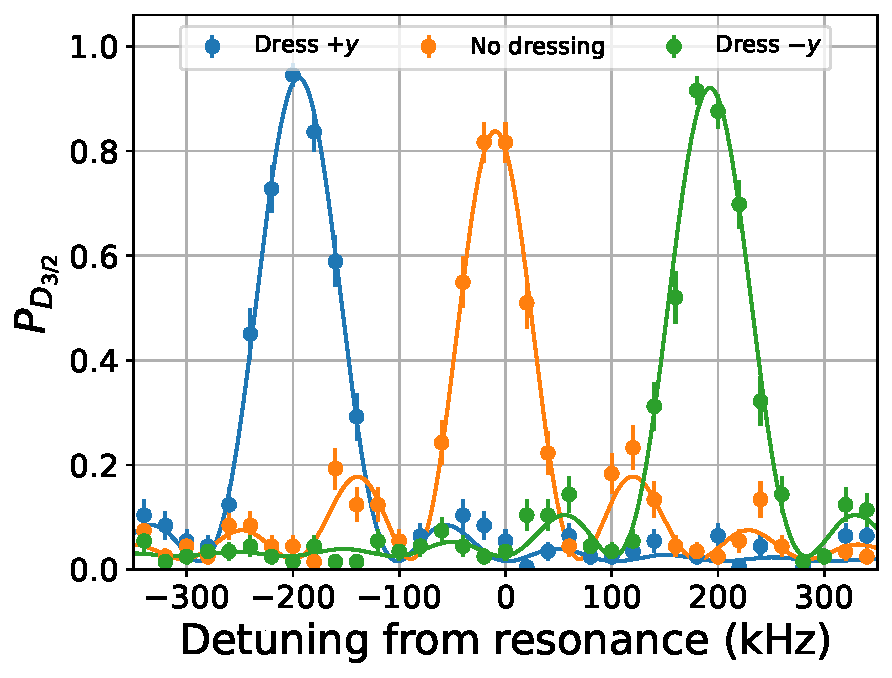
\includegraphics[width=18cm]{imgs/data_20240524_spec_dressed.pdf}};
          \end{tikzpicture}
        \end{center}
      \end{block}
      \begin{block}{Mid circuit measurement with selective shelving}
        \begin{center}
          \begin{tikzpicture}
            \fill[color=pyplotc0] (-12, -9.5) rectangle (-8, -7)
            node[white,pos=.5,align=center]
            {\small Selective\\\small Shelving};
            \fill[color=pyplotc0] (0, -9.5) rectangle (4, -7)
            node[white,pos=.5] {$R_{435}\left(\pi\right)$};
            \fill[color=pyplotc0] (12, -9.5) rectangle (16, -7)
            node[white,pos=.5,align=center]
            {\small Selective\\\small Unshelving};
            \draw[-{Stealth[length=15mm,width=7mm]},line width=5] (-14, -9.5) node[left] {Data} -- (20, -9.5);

            \fill[color=pyplotc4] (-12, -13) rectangle (-8, -10.5)
            node[white,pos=.5,align=center] {\small Raman\\\small Dressing};
            \fill[color=cyan] (-7, -13) rectangle (11, -10.5)
            node[white,pos=.5] {Detection};
            \fill[color=pyplotc4] (12, -13) rectangle (16, -10.5)
            node[white,pos=.5,align=center] {\small Raman\\\small Dressing};
            \draw[-{Stealth[length=15mm,width=7mm]},line width=5] (-14, -13) node[left] {Aux} -- (20, -13);

            \draw[loosely dashed, line width=4.5, opacity=0.5] (-3.5, -14) -- (-3.5, -6.5);

            \node[text width=16cm,align=center] at (11, -21) {
              \begin{itemize}
              \item Detect auxiliary qubit without affecting shelved data qubit
              \item Use spin-echo on $435$~nm to improve coherence.
              \item Unshelve after detection to measure coherence/
                recover circuit operation.
              \end{itemize}
            };

            \begin{scope}[shift={(-9, -25)}]
              \begin{scope}[shift={(-5, 0)}]
                \node[above] at (1.5, 6.5) {Data};

                \draw[line width=2] (-0.5, 0) node[left] {$|1\rangle$} -- (0.5, 0);
                \draw[line width=2] (-0.5, -2.5) node[left] {$|0\rangle$} -- (0.5, -2.5);
                \draw[line width=2] (1, 1.5) -- (2, 1.5) node[right] {$|D\rangle$};

                \mytweezer.drawUpAtom(0, -2.5, 0.5)
                \mytweezer.drawDownAtom(1.5, 1.5, 0.5)
              \end{scope}
              \draw[line width=5,opacity=0.45] (0, 6) -- (0, -3.5);
              \begin{scope}[shift={(3.5, 0)}]
                \node[above] at (-0.5, 6.5) {Aux};
                \draw[line width=2] (-0.5, 5.5) node[left] {$|P\rangle$} -- (0.5, 5.5);

                \draw[line width=2] (-0.5, 0) node[left] {$|1\rangle$} -- (0.5, 0);
                \draw[line width=2] (-0.5, -2.5) node[left] {$|0\rangle$} -- (0.5, -2.5);

                \draw[cyan,-{Stealth[length=7mm,width=4mm]},line width=3] (-0.32, 0) -- (-0.32, 5.5);
                \draw[cyan,-{Stealth[length=7mm,width=4mm]},line width=3,
                decorate, decoration={pre length=0cm,
                  post length=4mm, snake, amplitude=1mm,
                  segment length=4mm}] (0.32, 5.5) -- (0.32, 0);

                \mytweezer.drawUpAtom(0, 0, 0.5)
                \mytweezer.drawDownAtom(0, -2.5, 0.5)
              \end{scope}
              \draw[rounded corners=0.5cm, line width=3, opacity=0.3] (-8, -4.2) rectangle (5, 8);
            \end{scope}

            \draw[-{Stealth[length=6mm,width=3.5mm]},line width=3]
            (-10.5, -17) -- (-10.5, -15.5) -| (-3.5, -14);
          \end{tikzpicture}
        \end{center}
      \end{block}
    \end{column} % End of the second column

    \begin{column}{\sepwid}
      \begin{center}
        {\color{gray}\rule{3pt}{\textheight}}
      \end{center}
    \end{column} % Empty spacer column

    \begin{column}{\colthreewid} % The third column
      \begin{block}{Preliminary results}
      \end{block}
      \begin{block}{Future works}
        \begin{itemize}
        \item Improve dressing and shelving fidelity
        \item Shelve to longer lived F$_{7/2}$ state for better protection
          {\scriptsize (Nature Physics vol. 18, 1058-1061 (2022))}
        \end{itemize}
        \begin{tikzpicture}[scale=1]
          % S1/2
          % F=1
          \draw[line width=2] (-1.8, 2) -- (-0.8, 2);
          \draw[line width=2] (-0.5, 2) -- (0.5, 2);
          \draw[line width=2] (0.8, 2) -- (1.8, 2);
          % F=0
          \draw[line width=2] (-0.5, 0) -- (0.5, 0);

          \coordinate (S1) at (0, 2);
          \coordinate (S0) at (0, 0);

          \node[left] at (-1.8, 2) {\small $F=1$};
          \node[left] at (-1.8, 0) {\small $F=0$};

          \mytweezer.drawUpAtom(0, 2, 0.5)
          \mytweezer.drawDownAtom(0, 0, 0.5)

          \node[left] at (-4.5, 1) {\small $^2\mathrm{S}_{1/2}$};

          % D5/2
          \begin{scope}[shift={(6.5, 7)}]
            % F=3
            \draw[line width=2] (-4.4, 1.2) -- (-3.4, 1.2);
            \draw[line width=2] (-3.1, 1.2) -- (-2.1, 1.2);
            \draw[line width=2] (-1.8, 1.2) -- (-0.8, 1.2);
            \draw[line width=2] (-0.5, 1.2) -- (0.5, 1.2);
            \draw[line width=2] (0.8, 1.2) -- (1.8, 1.2);
            \draw[line width=2] (2.1, 1.2) -- (3.1, 1.2);
            \draw[line width=2] (3.4, 1.2) -- (4.4, 1.2);
            % F=2
            \draw[line width=2] (-3.1, 0) -- (-2.1, 0);
            \draw[line width=2] (-1.8, 0) -- (-0.8, 0);
            \draw[line width=2] (-0.5, 0) -- (0.5, 0);
            \draw[line width=2] (0.8, 0) -- (1.8, 0);
            \draw[line width=2] (2.1, 0) -- (3.1, 0);

            \coordinate (D1) at (0, 1.2);
            \coordinate (D0) at (0, 0);

            \node[right] at (4.4, 1.2) {\small $F=3$};
            \node[right] at (4.4, 0) {\small $F=2$};

            \node[right] at (7.1, 0.6) {\small $^2\mathrm{D}_{5/2}$};
          \end{scope}

          % F7/2
          \begin{scope}[shift={(19, 2)}]
            % F=4
            \draw[line width=2] (-5.7, 1) -- (-4.7, 1);
            \draw[line width=2] (-4.4, 1) -- (-3.4, 1);
            \draw[line width=2] (-3.1, 1) -- (-2.1, 1);
            \draw[line width=2] (-1.8, 1) -- (-0.8, 1);
            \draw[line width=2] (-0.5, 1) -- (0.5, 1);
            \draw[line width=2] (0.8, 1) -- (1.8, 1);
            \draw[line width=2] (2.1, 1) -- (3.1, 1);
            \draw[line width=2] (3.4, 1) -- (4.4, 1);
            \draw[line width=2] (4.7, 1) -- (5.7, 1);
            % F=3
            \draw[line width=2] (-4.4, 0) -- (-3.4, 0);
            \draw[line width=2] (-3.1, 0) -- (-2.1, 0);
            \draw[line width=2] (-1.8, 0) -- (-0.8, 0);
            \draw[line width=2] (-0.5, 0) -- (0.5, 0);
            \draw[line width=2] (0.8, 0) -- (1.8, 0);
            \draw[line width=2] (2.1, 0) -- (3.1, 0);
            \draw[line width=2] (3.4, 0) -- (4.4, 0);

            \coordinate (F1) at (0, 1);
            \coordinate (F0) at (0, 0);

            \node[right] at (5.7, 1) {\small $F=4$};
            \node[right] at (5.7, 0) {\small $F=3$};

            \mytweezer.drawUpAtom(0, 1, 0.5)
            \mytweezer.drawDownAtom(0, 0, 0.5)

            \node[right] at (8.4, 0.5) {\small $^2\mathrm{F}_{7/2}$};
          \end{scope}

          \draw[-{Stealth[length=6mm,width=4.5mm]},pyplotc0,line width=2]
          (S0) -- (D1);
          \draw[-{Stealth[length=6mm,width=4.5mm]},pyplotc0,line width=2]
          (D1) -- (F0);

          \draw[-{Stealth[length=6mm,width=4.5mm]},pyplotc1,line width=2]
          (S1) -- (D0);
          \draw[-{Stealth[length=6mm,width=4.5mm]},pyplotc1,line width=2]
          (D0) -- (F1);
        \end{tikzpicture}
      \end{block}
    \end{column} % End of the third column
  \end{columns} % End of all the columns in the poster
\end{frame} % End of the enclosing frame

\end{document}
